\documentclass[11pt]{article}


% --- Packages ---
\usepackage{amsmath, amsthm, amsfonts, amssymb, hyperref, soul, latexsym, stmaryrd, booktabs} % fonts and characters
\usepackage{enumitem, ytableau, comment, graphicx, makecell, appendix, titling, scrextend, float, subcaption} % utilities
\usepackage{tikz, tikz-cd, tikzsymbols, pgfplots} % plots crap
\pgfplotsset{compat=1.18}
\usepackage{blkarray} % random math 
\usepackage{pstricks,pst-node,pst-tree} % networks
\usepackage{verbatim} % write code
\newlength\myverbindent % indent code
\setlength\myverbindent{0.5in} % change this to change indentation
\makeatletter
\def\verbatim@processline{%
  \hspace{\myverbindent}\the\verbatim@line\par}


% --- Formatting ---
\usepackage{fullpage} % margins

\numberwithin{equation}{section} % number equations with section number
\numberwithin{figure}{section} % number figure with section number
\numberwithin{table}{section} % number table with section number

\theoremstyle{definition}
\newtheorem{theorem}{Theorem}[section]
\newtheorem{lemma}[theorem]{Lemma}
\newtheorem{claim}[theorem]{Claim}
\newtheorem{conjecture}[theorem]{Conjecture}
\newtheorem{proposition}[theorem]{Proposition}
\newtheorem{corollary}[theorem]{Corollary}
\newtheorem{problem}[theorem]{Problem}
\newtheorem{exercise}[theorem]{Exercise}
\newtheorem{definition}[theorem]{Definition}

\newenvironment{solution}{\begin{addmargin}[2em]{0em} {\bf Solution. }}{\end{addmargin}}


% --- Math Crap ---
\newcommand{\E}{\mathbb{E}}
\newcommand{\Z}{\mathbb{Z}}
\newcommand{\R}{\mathbb{R}}
\newcommand{\Q}{\mathbb{Q}}
\newcommand{\C}{\mathbb{C}}
\newcommand{\N}{\mathbb{N}}
\newcommand{\lagr}{\mathcal{L}}
\newcommand{\e}{\varepsilon}
\renewcommand{\sup}{\text{sup}}
\renewcommand{\inf}{\text{inf}}
\renewcommand{\d}{\delta}
\renewcommand{\Re}{\text{Re}}
\renewcommand{\Im}{\text{Im}}
\newcommand{\Arg}{\text{Arg}}
\newcommand{\Log}{\text{Log}}
\newcommand{\conj}{\overline}
\newcommand{\intersection}{\cap}
\newcommand{\union}{\cup}


% --- Bibliography ---
\usepackage[authordate, backend=biber, ibidtracker=false]{biblatex-chicago} % packages
\bibliography{key_bridge.bib} % .bib file


% --- Title ---
\title{Vulnerability of Urban Road Systems \\ %
    \large A Network Analysis of the Baltimore Bridge Collapse}
\author{Gavin Engelstad}
\date{Spring 2024}


% --- Document ---
\begin{document}
\maketitle

\begin{abstract}
    I have absolutely no idea what will go here, but I'll sure as hell put something.
\end{abstract}

\section{Introduction}

On March 26, 2024, the container ship Dali struck one of the concrete supports holding up the Francis Scott Key Bridge and caused it to collapse. The incident caused six deaths\footnote{Only four of the six bodies have been found. Still, the remaining two were on the bridge during the collapse and are presumed dead \parencite{Hassan24}.} and caused trade through the port of Baltimore, one of the largest ports in the country, to grind to a halt costing an estimated \$15 million per day \parencites{Hassan24}{AlJazeera24}.

Pre-collapse, the Francis Scott Key Bridge was an essential part of the Baltimore road system. It was the final link completed in Interstate 695, or the Baltimore Beltway, a major highway that wraps around the City of Baltimore. Spanning the Port of Baltimore, the bridge was 1.6 miles (2.6 km) across and the third-longest continuous truss bridge in the world \parencite{Parry24}. Every day, approximately 30 thousand vehicles crossed the bridge, making it an important piece of infrastructure for thousands of commuters every day \parencite{MDOT24}. Post collapse, the Maryland Department of Transportation issued a traffic warning and has observed a 7-11\% increase in traffic along alternate major highway routes across and around the port \parencites{MDOT24}{Domen24}.

% TODO results

This paper will examine the effects of the bridge collapse on the Baltimore Metro Area (BMA) road system using tools from complex network analysis. The rest of the paper will proceed as follows: Section \ref{sec:lit_review} will explore existing literature on the use of complex networks to analyze road network structures and robustness. Section \ref{sec:model} will outline the methods we'll use to analyze the effects of the bridge collapse on the road network. Section \ref{sec:data} will present the data sources that we'll use to create and examine the network. %  Section \ref{sec:results} will give the results to our analysis. Finally, section \ref{sec:concl} will conclude.


\section{Literature Review} \label{sec:lit_review}

Road systems have a long history of being represented as a network. The most popular method of this, the primal approach, uses intersections as nodes and roads as links in the network \parencites{Porta06}{Ding19}. This method is seen as more comprehensive, realistic, and feasible than the alternative dual approach to modeling the network \parencites{Porta06}{Porta06b}. This approach is implemented into many software packages and databases \parencites{Esri}{Boeing17} and has the advantage that it allows for analysis that considers distance, versus solely looking at the topological properties of the network \parencites{Ding19}{Erath09}{Wang11}{Barthelemy09}.

Using this network, centrality measures can be very predictive of the real world context around roads and intersections. Typically, multiple centrality assessment (MCA) methods that analyze a number of centrality measures are used to give a comprehensive view of the network \parencites{Porta06}{Porta07}. Closeness centrality, when done globally, is highly correlated with land-use, but fails to be meaningful looking at only a subset of a larger network \parencites{Wang11}{Porta06}{Barthelemy09}. Betweenness centrality is very effective at identifying important parts of longer routes to traverse large urban networks \parencite{Porta06}. Straightness centrality, a modification of closeness centrality where the distance along the network is divided the Euclidean distance between nodes, identifies both areas with high land-use and important routes while being robust on network subsets \parencites{Porta06}{Wang11}. Information centrality, which measures the drop in global efficiency when a piece of the network is removed, is a comprehensive measure of node importance and identifies nodes that have high centrality from all other measures \cite{Porta06}. Eigenvector centrality is able to identify high-traffic areas and road connectivity \parencites{Jayaweera17}{Ando21}.

These tools are useful to analyze network robustness. On its own, eigenvector centrality can identify nodes in a network that are vulnerable to the removal of other nodes \parencite{Ando20}. Analysis of how stable centrality measures are when nodes are added or removed, a technique called centrality interference or centrality robustness, can act as a measure of road network robustness \parencite{Scardoni13}.

Other tools to analyze road network robustness look at the topological properties of the network after an attack, defined as the removal of edges or nodes in the network \parencite{Holme02}. The clustering coefficient, serves as a measure of reliability of a network, and how much it changes after an attack can show how much the attack affects network connectivity \parencite{Xeumei10}. The change in the average shortest path also serves to demonstrate how robust people's ability to travel along the network is to an attack \parencites{Xeumei10}{Kaub24}.

This paper will implement these methods on the Baltimore road network, utilizing MCA combined with centrality interference methods and analyzing how the average shortest path changes before versus after the bridge was destroyed. Most studies that implement these methods do so at a theoretical level and attempt to identify the edges and nodes where the network is most vulnerable to an attack \parencites{Xeumei10}{Ando21}{Masuccia16}{Julliard15}{Holme02}. The handful of studies that implement these methods that are inspired by real events tend to analyze the effects of disasters that have affects that span the entire network \parencites{Kaub24}{Sakakibara04}. Therefore, this paper's application of these methods to the real-world removal of a single, important edge of a city's road network is, to my knowledge, new.


\section{Model} \label{sec:model}

\subsection{Network Structure}

The first way we'll analyze the robustness of the network is through comparing the structure of the network before versus after the destruction of the bridge.

At a global scale, that means we'll be comparing the average path between nodes. To calculate this, we'll use
\[
  \overline{d} = \frac{1}{n(n-1)} \sum_{i \in N} \sum_{j \in N, j \neq i} d_{i, j}
\]
where $n$ is the number of nodes in the network, $N$ is the set of all nodes in the network, and $d_{i, j}$ is the distance between nodes $i$ and $j$ traveling along the network. This will tell us how far an individual has to travel to get from one randomly chosen intersection to another. Any change in this that we observe would suggest the bridge collapse has made it harder to travel across the network, though, since the event only affected a small part of the road network, we don't expect any observed change to be particularly significant.

Because of this likely smaller global effect, we also want to study the local effects of the bridge collapse within the network. Therefore, we'll also look at node level centrality measures and node-node pair level travel lengths.

For centrality measures, we'll look at the eigenvector centrality ($C^E_i$), betweenness centrality ($C^B_i$), closeness centrality ($C^C_i$), and straightness centrality ($C^S_i$). The first three of these are standard in complex network analysis and tell us whether a node is connected to important nodes ($C^E_i$), between other nodes ($C^B_i$), and close to other nodes ($C^B_i$). For $C_i^E$, we'll follow \cite{Ando20}, where roads were weighted based on capacity, and weight edges based on the type of road they represent. For $C^B_i$ and $C^C_i$, we'll weight edges by their lengths.

Straightness centrality is a measure specific to the study of spacial networks, networks where the nodes and edges have a physical location, that tells us how directly a node can get to other nodes along the network. Introduced in \cite{Porta06}, it's calculated using 
\[
  C_i^S = \frac{1}{n-1} \sum_{j \in N, j \neq i} \frac{d_{i, j}^\text{Eucl}}{d_{i, j}}
\]
where $d_{i, j}^\text{Eucl}$ is the Euclidean distance between the points. Intuitively, a straightness centrality of 1 implies a node has a straight connection to all other nodes along the network, and anything lower tells us how inefficient traveling along the network is relative to just taking the straightest route.

To use these centrality measures to analyze robustness, we'll analyze how much they change when the Key Bridge is removed from the network. This gives us a method of analyzing how individual nodes on the network were affected by the bridge collapse and where the most affected nodes are located.

To get an even more specific look at the implications of the collapse, we'll also look at how travel lengths between individual nodes are affected. To do this we'll compare $d_{i, j}$ for all $i, j \in N$ to see which routes were the most affected and what areas of the city these routes go through. This will help give us an idea of which trips the blockage will impact, and, therefore, the types of people that will be the most affected by the blockage.


\subsection{Network Utilization}

Analysis of the overall structure of the Baltimore road system will give us a general idea of how the network, nodes, and paths were affected by the bridge collapse, but it doesn't take into account how people actually use the road network. People aren't evenly spread throughout a city and equally likely start and end their journeys at all nodes.

To fix this, we'll use commute data to weight trips based on how often the routes are actually being traveled. Using this new measure, we'll look at the average shortest path length and equivalences to betweenness, closeness, and straightness centrality.

Our utilization-sensitive shortest path length will be calculated as
\[
  \overline{d} = \frac{1}{\sum_{i \in N} \sum_{j \in N, j \neq i} n_{i, j}} \sum_{i \in N} \sum_{j \in N, j \neq i} n_{i, j} d_{i, j}
\]
where $n_{i, j}$ is the number of people traveling from node $i$ to $j$.

Use-weighted betweenness centrality will be calculated as
\[
  C_i^B = \frac{1}{\sum_{j \in N, j \neq i} \sum_{k \in N, k \neq i, j} n_{j, k}} \sum_{j \in N, j \neq i} \sum_{k \in N, k \neq i, j} n_{j, k} \frac{p_{j, k} (i)}{p_{j, k}}
\]
where $p_{j, k}$ is the number of shortest paths between $j$ and $k$ and $p_{j, k} (i)$ us the number of shortest paths between $j$ and $k$ that cross $i$. Therefore, we're measuring the number of traveled paths that go through $i$, not just possible paths like with normal betweenness centrality.

Use-weighted closeness centrality will be
\[
  C_i^C = \frac{\sum_{j \in N, j \neq i} n_{i, j}}{\sum_{j \in N, j \neq i} n_{i, j} d_{i, j}}.
\]
The interpretation of this is a measure of how far individuals starting at $i$ need to travel.

Finally, use-weighted straightness centrality will be
\[
  C_i^S = \frac{1}{\sum_{j \in N, j \neq i} n_{i, j}} \sum_{j \in N, j \neq i} n_{i, j} \frac{d_{i, j}^\text{Eucl}}{d_{i, j}}.
\]
This can be interpreted as how direct the paths of individuals starting at $i$ are.

Together, this will give us tools to analyze the ways the collapse affected how people use the road system in the Baltimore Metro Area, not just the structure of the network.


\section{Data} \label{sec:data}

For our analysis, we'll use a road system from Open Street Maps provided by the Python API from \cite{Boeing17}. This API allows us to get a directed network of roads and intersections for almost anywhere in the world, along with basic statistics about each section of road, like the exact coordinates, length, road type, and number of lanes. 

In our study, we'll focus on the 7 counties that make up the Baltimore metro area: Anne Arundel, Baltimore City, Baltimore County, Carroll, Harford, Howard, and Queen Anne's. To make our analysis feasible and meaningful, especially the eigenvector centrality and average shortest path, we exclude any intersections that aren't strongly connected to the largest connected component. This results in us excluding 272 intersections in the network, mostly near the county boundaries.

The resulting network has 91,300 intersections (nodes) and 218,842 road segments (edges), 4 of which are on the Key Bridge and were affected by the collapse. A visualization of this network is shown in Figure \ref{fig:network}. We can see the road network varies substantially in density, and is much denser near the city and to the South nearer to Washington DC. The zoomed in view of the Key Bridge shows the bridge plays an important role in the network. When the bridge is removed, paths that normally go across it will need to be diverted moderately far West towards downtown. Therefore, we can expect a significant number of shortest paths to be rerouted and affected.

\begin{figure}[t]
	\caption{Baltimore Metro Area Road Network}
  \begin{subfigure}{0.49\textwidth}
    \centering
    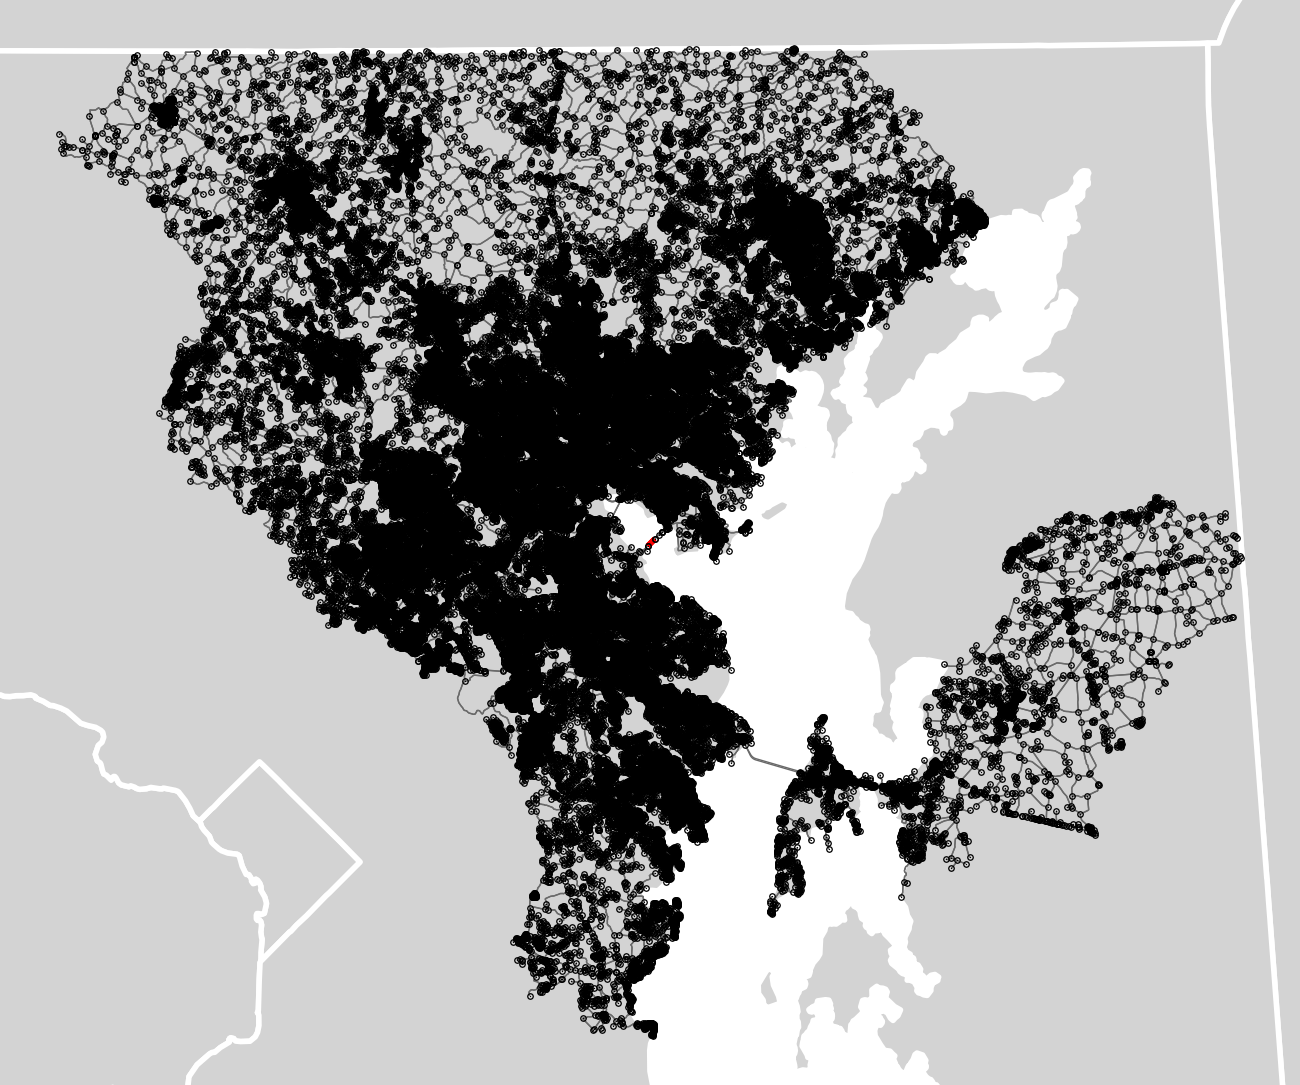
\includegraphics[width=\textwidth]{maps/full_network.png}
    \caption{Total BMA Network}
  \end{subfigure}
  \begin{subfigure}{0.49\textwidth}
    \centering
    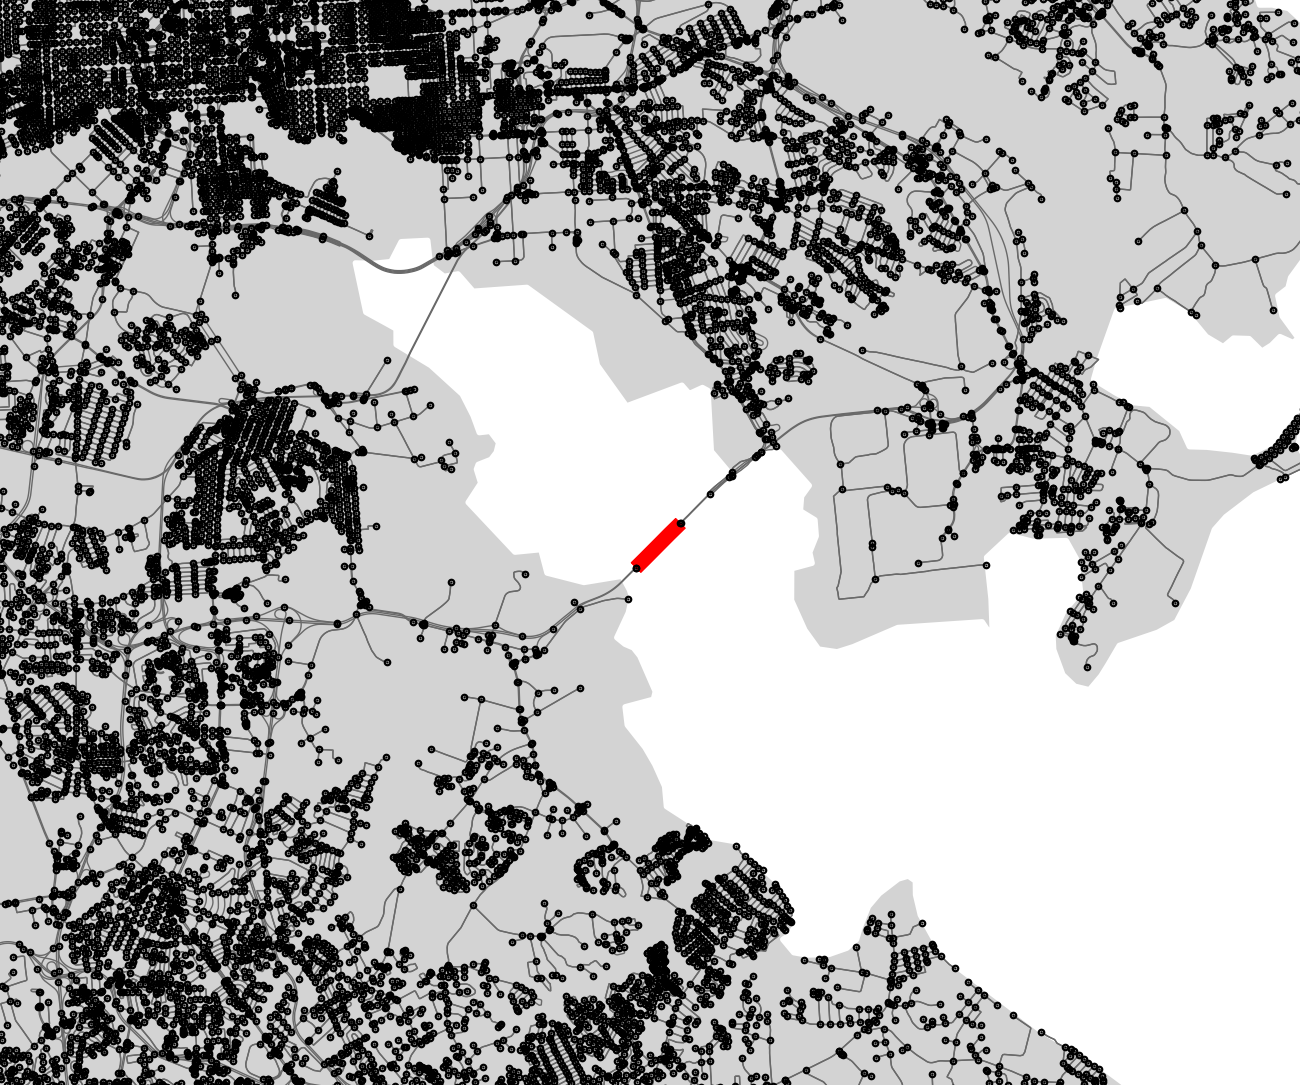
\includegraphics[width=\textwidth]{maps/zoomed_network.png}
    \caption{Zoomed In to Key Bridge}
  \end{subfigure}

  \begin{center}
    {\footnotesize \emph{Note:} Key Bridge highlighted in red.}
  \end{center}
  \label{fig:network}
\end{figure}

For data on network utilization, we'll use census tract level journey-to-work flows from the US CENSUS \parencite{Bolton20}. This data gives bilateral flow estimates for the number of daily commuters from each census tract to every other census tract from 2012 to 2016. This isn't the time period we're interested in, but is the most recent data available. Due to the bounds of the road network we're working with, we only include commuters who both live and work within the BMA. This excludes 11.1\% of commuters who work in the BMA and 12.2\% of commuters who live in the BMA.

The dataset includes 678 tracts within the BMA. 672 of these are home to at least one commuter and all 678 are the workplace of at least one commuter. Together, there are 41,272 residence-workplace pairs which 1.02 million commuters travel between. The maps in Figure \ref{fig:tracts} shows the commuter volume into and from census tracts in the BMA. We can see that commuter residences are somewhat evenly distributed throughout the area, but workplaces are much more central. When we calculate paths commuters are taking along the network, this will mean that the paths will point to a much more central location, which may limit how many go across the relatively off to the side Key Bridge. The density plot in Figure \ref{fig:tracts} shows that commuter flow has a significant right-skew which even appears on a log-scale plot. This means that commuter flows are, typically, fairly low, but there are tract pairs with much higher flow.

\begin{figure}[t!]
	\caption{Baltimore Metro Area Census Tracts by Commuter Volume and Flow}
  \begin{subfigure}{0.49\textwidth}
    \centering
    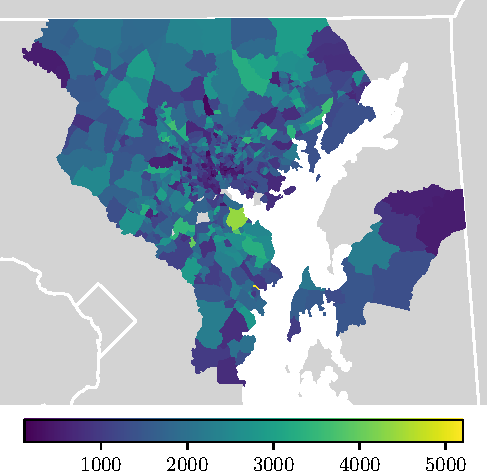
\includegraphics[width=\textwidth]{maps/tract_home.pdf}
    \caption{Commuter Homes}
  \end{subfigure}
  \begin{subfigure}{0.49\textwidth}
    \centering
    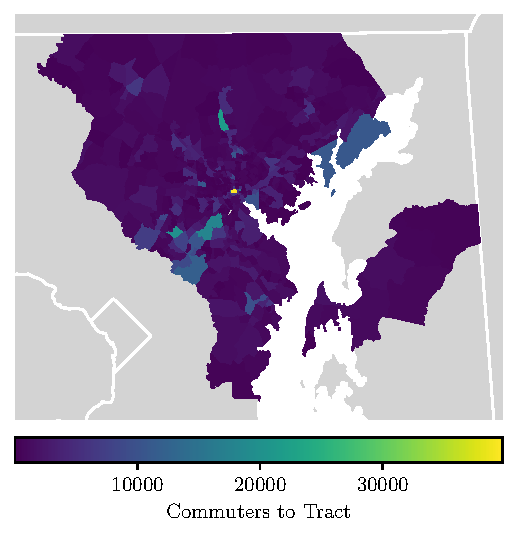
\includegraphics[width=\textwidth]{maps/tract_work.pdf}
    \caption{Commuter Workplaces}
  \end{subfigure}
  \begin{subfigure}{\textwidth}
    \centering
    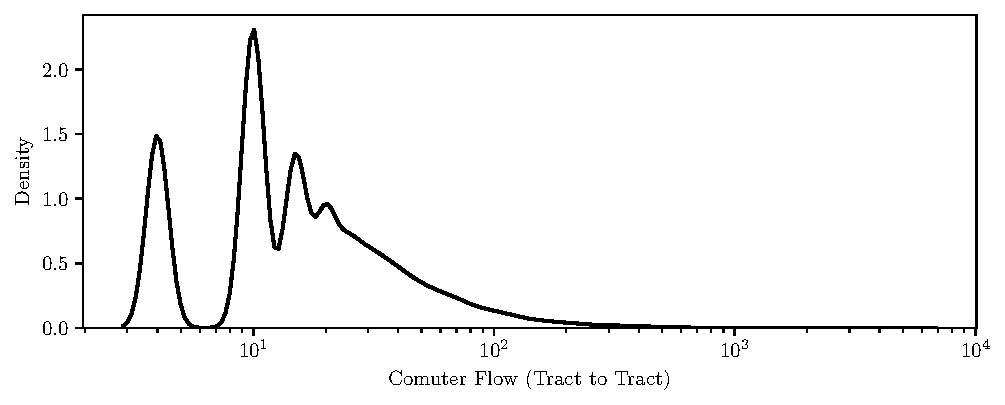
\includegraphics[width=\textwidth]{graphs/tract_flows.pdf}
    \caption{Tract to Tract Bilateral Commuter Flows}
  \end{subfigure}

  \label{fig:tracts}
\end{figure}

We are limited by the granularity of this data. Census tracts are very large compared to the intersection/road segment scale of the network, which means we can't perfectly estimate the paths commuters are taking.\footnote{But definitely is a positive from a privacy standpoint.} In our analysis, we'll estimate paths with commuters starting and ending at the intersection closest to the center-of-mass of the census tracts they're traveling between and assuming all commuters travel along the road network. This should give us a reasonably accurate estimate for how commuters are traveling, although will have some errors, especially closer to the center of mass for the higher-volume census tracts.



\section{Results} \label{results}



% \section{Conclusion} \label{sec:concl}

% limitations:
% no cascade model: there wouldn't be a cascade
% no lcc, clustering, etc: aren't affected
% arbitrary boundry
% high trip spread


\clearpage
\printbibliography



\end{document}